\documentclass[tikz,border=9pt]{standalone}
\usepackage[scaled=0.95]{helvet}
\renewcommand{\familydefault}{\sfdefault}
\usepackage[europeanresistors,americanvoltages]{circuitikz}
\definecolor{TEJNavy}{HTML}{1E2B55}
\definecolor{TEJBlue}{HTML}{1769AA}
\begin{document}
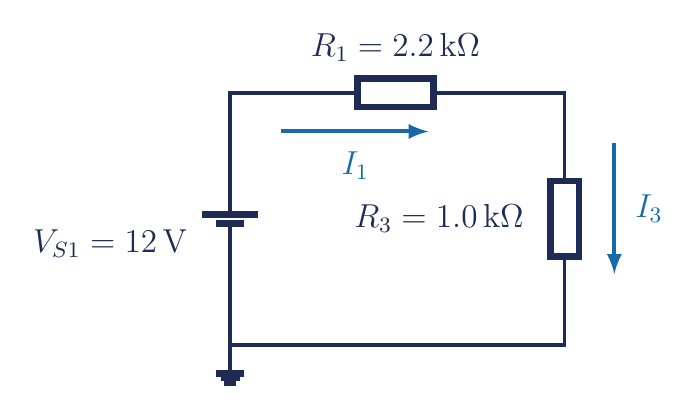
\begin{tikzpicture}[line width=1.2pt,draw=TEJNavy,text=TEJNavy,>=latex]
  \ctikzset{bipoles/length=1.2cm}
  \draw (0.8,0.8) to[battery1,invert] (0.8,4.0)
    -- (1.55,4.0) to[R] (4.25,4.0) -- (5.05,4.0)
    to[R] (5.05,0.8) -- (0.8,0.8);
  \draw (0.8,0.8) node[ground] {};
  \node[fill=white,inner sep=2pt,font=\large] at (2.90,4.58)
    {$R_1=2.2\,\mathrm{k}\Omega$};
  \node[fill=white,inner sep=2pt,font=\large,anchor=east] at (4.62,2.40)
    {$R_3=1.0\,\mathrm{k}\Omega$};
  \node[fill=white,inner sep=2pt,font=\large,anchor=east] at (0.35,2.08)
    {$V_{S1}=12\,\mathrm{V}$};
  \draw[->,TEJBlue,line width=1.45pt] (1.45,3.51) -- (3.32,3.51);
  \node[fill=white,inner sep=2pt,font=\large,text=TEJBlue] at (2.39,3.08) {$I_1$};
  \draw[->,TEJBlue,line width=1.45pt] (5.68,3.36) -- (5.68,1.70);
  \node[fill=white,inner sep=2pt,font=\large,text=TEJBlue] at (6.12,2.53) {$I_3$};
\end{tikzpicture}
\end{document}
